\section{Nguyên lý thiết kế hệ thống}\label{sec:design-principles}

\subsection{Tổng quan}\label{sec:dp-overview}
\begin{table}[H]
\centering
\caption{Các nhóm nguyên tắc thiết kế}\label{tab:dp-groups}
\small
\renewcommand{\arraystretch}{1.3}
\begin{tabularx}{\textwidth}{|>{\raggedright\arraybackslash}p{4.6cm}|>{\raggedright\arraybackslash}p{3.8cm}|>{\raggedright\arraybackslash}X|}
\hline
\textbf{Nhóm} & \textbf{Đặc tính phục vụ} & \textbf{Nguyên tắc} \\
\hline
Độ tin cậy và toàn vẹn dữ liệu & Reliability, Data Integrity & DP-01 -- DP-04 \\
\hline
Hiệu năng và tự chủ khi mất kết nối & Performance, Availability & DP-05 -- DP-09 \\
\hline
Bảo mật và bảo vệ dữ liệu cá nhân & Security, Privacy, Auditability & DP-10 -- DP-13 \\
\hline
Tính module và khả năng sửa đổi & Modifiability, Scalability & DP-14 -- DP-17 \\
\hline
\end{tabularx}
\end{table}

%==============================================================================
\subsection{Nhóm nguyên tắc về độ tin cậy và toàn vẹn dữ liệu}\label{sec:dp-reliability}
Nhóm này phục vụ hai trong ba đặc tính dẫn dắt của hệ thống (Mục~\ref{sec:top3}): không để mất và không để sai lệch dữ liệu chấm công.

\paragraph{DP-01. Lưu bền vững trước khi xác nhận.}\label{dp:01}
\begin{itemize}
    \item \textit{Phát biểu:} Không thông báo thành công cho một thao tác khi dữ liệu của thao tác đó chưa được lưu bền vững, hoặc khi bên thực hiện cuối cùng chưa xác nhận.
    \item \textit{Lý do:} NFR-REL-03, NFR-AVL-03, INV-05; Reliability.
    \item \textit{Áp dụng trong TMC:} trong luồng F1, G1 ghi lượt quét ở trạng thái chờ xác nhận trước khi gọi cổng xoay, và chỉ ghi giao dịch chấm công cùng bản ghi outbox khi cổng đã xác nhận mở (ADR-03). C4 ghi đợt truyền trước khi C5 gửi đi; kỳ chỉ chuyển sang LOCKED khi HR/Payroll xác nhận.
    \item \textit{Trường hợp linh hoạt:} dữ liệu có thể dựng lại được, như read model của C6 hoặc heartbeat, không cần ghi trước khi xử lý.
\end{itemize}

\paragraph{DP-02. Dữ kiện bất biến, sửa bằng bản ghi mới.}\label{dp:02}
\begin{itemize}
    \item \textit{Phát biểu:} Dữ kiện đã ghi nhận (giao dịch chấm công, nhật ký kiểm toán) không bị sửa hay xóa; mọi thay đổi được thể hiện bằng một bản ghi mới tham chiếu tới bản ghi gốc.
    \item \textit{Lý do:} INV-08, INV-10; NFR-DIN-03; Data Integrity, Auditability.
    \item \textit{Áp dụng trong TMC:} AttendanceTransaction và AuditLogEntry chỉ được ghi thêm; việc sửa chấm công dùng AttendanceAdjustment; sau khi kỳ chuyển sang LOCKED, thay đổi được gửi qua đợt truyền bổ sung (INV-09). ScanAttempt chỉ được đổi trạng thái theo đúng vòng đời: chờ xác nhận, rồi được chấp nhận hoặc mở cổng thất bại.
    \item \textit{Trường hợp linh hoạt:} dữ liệu danh mục như hồ sơ nhân viên và cấu hình trạm được cập nhật tại chỗ, nhưng mỗi thay đổi phải được ghi nhật ký kiểm toán.
\end{itemize}

\paragraph{DP-03. Idempotent cho mọi thao tác có thể lặp lại.}\label{dp:03}
\begin{itemize}
    \item \textit{Phát biểu:} Mọi thao tác có thể bị gửi lại hoặc xử lý lại phải cho cùng một kết quả, không tạo bản ghi trùng.
    \item \textit{Lý do:} NFR-DIN-02, NFR-INT-04, INV-06; Data Integrity.
    \item \textit{Áp dụng trong TMC:} mã sự kiện được sinh tại cổng và C1 bỏ qua bản ghi trùng; mỗi đợt truyền HR/Payroll có mã đợt; việc đồng bộ nhân viên cập nhật theo mã nhân viên (ADR-09); trước khi gửi lại lệnh mở cổng, G2 kiểm tra trạng thái cổng (ADR-06).
    \item \textit{Trường hợp linh hoạt:} thao tác chỉ đọc vốn đã idempotent, không cần cơ chế chống trùng.
\end{itemize}

\paragraph{DP-04. Mỗi loại dữ liệu chỉ có một nơi sở hữu.}\label{dp:04}
\begin{itemize}
    \item \textit{Phát biểu:} Mỗi loại dữ liệu chỉ được ghi bởi đúng một component; component khác chỉ đọc qua interface của component sở hữu hoặc nhận bản sao chỉ đọc.
    \item \textit{Lý do:} Data Integrity; tránh xung đột khi ghi và giữ được ranh giới giữa các module và quantum.
    \item \textit{Áp dụng trong TMC:} cột \textit{Dữ liệu sở hữu} ở Bảng~\ref{tab:components}; HR/Payroll sở hữu dữ liệu nhân sự gốc, C2 chỉ giữ bản đồng bộ; bản sao credential trong G3 chỉ được G4 cập nhật, G1 chỉ đọc.
    \item \textit{Trường hợp linh hoạt:} read model của C6 là dữ liệu dẫn xuất, có thể dựng lại từ dữ liệu gốc.
\end{itemize}

Nhóm nguyên tắc này bảo đảm rằng khi xảy ra mất kết nối hoặc gián đoạn giữa chừng, dữ liệu chấm công không bị mất (DP-01) và việc gửi bù không tạo dữ liệu trùng (DP-03).

%==============================================================================
\subsection{Nhóm nguyên tắc về hiệu năng và tự chủ khi mất kết nối}\label{sec:dp-autonomy}
Nhóm này phục vụ đặc tính dẫn dắt Performance và yêu cầu hoạt động khi mất kết nối, là cơ sở của Gate Quantum.

\paragraph{DP-05. Cổng tự chủ.}\label{dp:05}
\begin{itemize}
    \item \textit{Phát biểu:} Đường xử lý một lượt quét chỉ được dùng dữ liệu và thành phần nằm trong nhà máy; không có lời gọi đồng bộ nào tới trung tâm trên đường này.
    \item \textit{Lý do:} NFR-PER-01, FR-17, NFR-AVL-04; tiêu chí K4.
    \item \textit{Áp dụng trong TMC:} G1 xác thực mã QR bằng bản sao credential và khóa công khai trong G3 (ADR-01, ADR-02).
    \item \textit{Trường hợp linh hoạt:} các thao tác nằm ngoài luồng quét, như cấp mã QR, tra cứu báo cáo và quản trị, được gọi đồng bộ tới trung tâm.
\end{itemize}

\paragraph{DP-06. Bất đồng bộ cho việc không cần kết quả ngay.}\label{dp:06}
\begin{itemize}
    \item \textit{Phát biểu:} Việc nào người dùng không chờ kết quả thì được đưa ra khỏi luồng xử lý chính và thực hiện bất đồng bộ.
    \item \textit{Lý do:} NFR-PER-01, NFR-INT-02.
    \item \textit{Áp dụng trong TMC:} đồng bộ giữa hai quantum qua outbox; truyền dữ liệu HR/Payroll theo lô; cập nhật read model qua sự kiện; không dùng message broker (ADR-05).
    \item \textit{Trường hợp linh hoạt:} lệnh mở cổng và kiểm tra quyền luôn đồng bộ vì người dùng đang chờ kết quả.
\end{itemize}

\paragraph{DP-07. Mọi lời gọi ra ngoài có giới hạn thời gian chờ và đường lùi.}\label{dp:07}
\begin{itemize}
    \item \textit{Phát biểu:} Mọi lời gọi tới hệ thống bên ngoài hoặc qua mạng phải có giới hạn thời gian chờ và một hành động thay thế được định nghĩa trước khi lời gọi thất bại.
    \item \textit{Lý do:} NFR-AVL-03, NFR-REL-01, NFR-REL-02; R-03.
    \item \textit{Áp dụng trong TMC:} lời gọi cổng xoay giới hạn 800 ms, kiểm tra trạng thái trước khi gửi lại, circuit breaker và mở cổng thủ công; truyền HR/Payroll gửi lại theo exponential backoff và cho phép gửi lại thủ công; khi nhân viên không lấy được mã QR, bảo vệ mở cổng thủ công (ADR-06).
    \item \textit{Trường hợp linh hoạt:} lời gọi trong cùng tiến trình giữa các module không cần giới hạn thời gian chờ riêng.
\end{itemize}

\paragraph{DP-08. An toàn khi lỗi.}\label{dp:08}
\begin{itemize}
    \item \textit{Phát biểu:} Khi không đủ thông tin để quyết định, hệ thống chọn trạng thái an toàn: chiều vào đóng, chiều ra mở; không báo thành công khi kết quả chưa chắc chắn.
    \item \textit{Lý do:} NFR-SEC-02, NFR-AVL-03; an toàn của người lao động khi có sự cố.
    \item \textit{Áp dụng trong TMC:} khi mất kết nối quá ngưỡng, chiều vào chỉ mở thủ công còn chiều ra luôn được phép (Bảng~\ref{tab:gate-connection-states}); khi cổng xoay không xác nhận, kiosk báo mở cổng thất bại.
    \item \textit{Trường hợp linh hoạt:} giá trị ngưỡng mất kết nối được cấu hình theo từng nhà máy tại C9.
\end{itemize}

\paragraph{DP-09. Quan sát được.}\label{dp:09}
\begin{itemize}
    \item \textit{Phát biểu:} Mỗi module cung cấp health check và các chỉ số vận hành đủ để phát hiện sự cố trước khi người dùng bị ảnh hưởng.
    \item \textit{Lý do:} FR-09, NFR-AVL-04; Availability.
    \item \textit{Áp dụng trong TMC:} heartbeat của trạm; chỉ số về số bản ghi chờ trong outbox, độ trễ đồng bộ, trạng thái circuit breaker và trạng thái đợt truyền; cảnh báo khi gần hạn 12:00 ngày 1 mà đợt truyền chính chưa được xác nhận.
    \item \textit{Trường hợp linh hoạt:} module chỉ đọc như C6 chỉ cần health check.
\end{itemize}

Đây là nhóm nguyên tắc giải quyết trực tiếp vấn đề mất kết nối: cổng không phụ thuộc trung tâm (DP-05, DP-06), mọi lời gọi ra ngoài đều có đường lùi (DP-07), hệ thống chọn trạng thái an toàn khi thiếu thông tin (DP-08) và sự cố được phát hiện sớm (DP-09).

%==============================================================================
\subsection{Nhóm nguyên tắc về bảo mật và bảo vệ dữ liệu cá nhân}\label{sec:dp-security}
Nhóm này áp dụng các đặc tính nền tảng Security, Privacy và Auditability xuyên suốt các component.

\paragraph{DP-10. Đặc quyền tối thiểu, kiểm tra quyền phía server.}\label{dp:10}
\begin{itemize}
    \item \textit{Phát biểu:} Mỗi vai trò chỉ có quyền tối thiểu cần cho công việc; quyền được kiểm tra phía server ở cả mức chức năng và mức dữ liệu.
    \item \textit{Lý do:} NFR-SEC-01, NFR-SEC-04, NFR-PRI-01, INV-11.
    \item \textit{Áp dụng trong TMC:} C7 kiểm tra quyền cho mọi API; giám sát sản xuất chỉ xem nhân viên thuộc bộ phận phụ trách; bảo vệ chỉ có quyền mở cổng thủ công tại nhà máy của mình (ADR-08).
    \item \textit{Trường hợp linh hoạt:} kiosk không yêu cầu tài khoản người dùng; việc cho qua dựa trên chữ ký của mã QR và chứng chỉ của thiết bị.
\end{itemize}

\paragraph{DP-11. Không tin dữ liệu đến từ biên.}\label{dp:11}
\begin{itemize}
    \item \textit{Phát biểu:} Mọi dữ liệu đến từ thiết bị hoặc kênh không do trung tâm kiểm soát phải được xác thực nguồn gốc và tính toàn vẹn; khóa bí mật chỉ được đặt tại trung tâm.
    \item \textit{Lý do:} NFR-SEC-02, NFR-SEC-05; R-06.
    \item \textit{Áp dụng trong TMC:} G1 kiểm tra chữ ký, thời hạn và tính dùng một lần của mã QR; Gate Agent xác thực với trung tâm bằng chứng chỉ thiết bị; C1 kiểm tra dữ liệu nhận được theo \textit{sync-contract}; khóa ký mã QR chỉ nằm tại C2 (ADR-02, ADR-08).
    \item \textit{Trường hợp linh hoạt:} kết nối tới cổng xoay trong VLAN cô lập tuân theo hợp đồng API của nhà cung cấp.
\end{itemize}

\paragraph{DP-12. Bảo vệ dữ liệu cá nhân từ thiết kế.}\label{dp:12}
\begin{itemize}
    \item \textit{Phát biểu:} Chỉ thu thập, lưu trữ, truyền và hiển thị dữ liệu cá nhân khi thật sự cần, và luôn bảo vệ dữ liệu đó khi lưu và khi truyền.
    \item \textit{Lý do:} C-03, NFR-PRI-01 -- NFR-PRI-04.
    \item \textit{Áp dụng trong TMC:} bản sao tại cổng chỉ chứa mã credential, mã nhân viên và trạng thái; dữ liệu được mã hóa khi lưu và khi truyền; chỉ gửi sang HR/Payroll các trường trong hợp đồng dữ liệu; thời hạn lưu được cấu hình tại C9; kiosk chỉ hiển thị mã nhân viên và kết quả.
    \item \textit{Trường hợp linh hoạt:} nhân viên HR được xem đầy đủ hồ sơ khi xử lý nghiệp vụ, và mỗi lần xem được ghi nhật ký kiểm toán.
\end{itemize}

\paragraph{DP-13. Mọi thao tác nhạy cảm đều để lại dấu vết kiểm toán.}\label{dp:13}
\begin{itemize}
    \item \textit{Phát biểu:} Mọi thao tác làm thay đổi quyền, dữ liệu chấm công, mã QR hoặc trạng thái ra vào phải được ghi nhật ký kiểm toán, kể cả khi thao tác diễn ra lúc mất kết nối.
    \item \textit{Lý do:} NFR-AUD-01 -- NFR-AUD-05, INV-10.
    \item \textit{Áp dụng trong TMC:} C8 chỉ ghi thêm và lưu chuỗi băm giữa các bản ghi; thao tác mở cổng thủ công được ghi cục bộ tại G3 rồi đồng bộ lên C8.
    \item \textit{Trường hợp linh hoạt:} các thao tác đọc thông thường không cần ghi nhật ký kiểm toán, trừ việc xem hồ sơ cá nhân đầy đủ.
\end{itemize}

Nguyên tắc DP-11 là cơ sở của giải pháp cho vấn đề mã QR tĩnh: mã QR chỉ được chấp nhận khi chứng minh được nguồn gốc bằng chữ ký của trung tâm, còn thời hạn ngắn và tính dùng một lần khiến mã bị lộ nhanh chóng mất giá trị.

%==============================================================================
\subsection{Nhóm nguyên tắc về tính module và khả năng sửa đổi}\label{sec:dp-modularity}
Nhóm này hướng dẫn cách tổ chức mã nguồn để hệ thống dễ thay đổi; cấu trúc module cụ thể được trình bày ở Mục~\ref{sec:module-views}.

\paragraph{DP-14. Phân rã theo domain, gắn kết cao.}\label{dp:14}
\begin{itemize}
    \item \textit{Phát biểu:} Mỗi module ứng với một subdomain hoặc một phần subdomain và chứa trọn vẹn dữ liệu, quy tắc và bất biến của phần đó.
    \item \textit{Lý do:} NFR-MOD-01; phân rã theo domain (Mục~\ref{sec:partitioning}).
    \item \textit{Áp dụng trong TMC:} mỗi package trong Bảng~\ref{tab:module-catalog} ứng với đúng một component; mỗi bất biến được bảo vệ trong một module, ví dụ INV-09 nằm trọn trong \texttt{period}.
    \item \textit{Trường hợp linh hoạt:} \texttt{sync-contract} là phần dùng chung giữa hai quantum.
\end{itemize}

\paragraph{DP-15. Ghép nối lỏng, không vòng phụ thuộc.}\label{dp:15}
\begin{itemize}
    \item \textit{Phát biểu:} Module chỉ phụ thuộc module khác qua interface công khai hoặc sự kiện, và đồ thị phụ thuộc giữa các module không có vòng.
    \item \textit{Lý do:} NFR-MOD-01; giữ khả năng triển khai độc lập của hai quantum.
    \item \textit{Áp dụng trong TMC:} \texttt{gate-agent} và \texttt{central} chỉ cùng phụ thuộc \texttt{sync-contract}; C1 gọi interface của C3 và C5 gọi interface của C2 để tránh vòng phụ thuộc (Hình~\ref{fig:module-uses}).
    \item \textit{Trường hợp linh hoạt:} \texttt{iam} và \texttt{audit} được mọi module nghiệp vụ dùng chung.
\end{itemize}

\paragraph{DP-16. Phụ thuộc hướng vào trong; hệ thống bên ngoài nằm sau adapter.}\label{dp:16}
\begin{itemize}
    \item \textit{Phát biểu:} Tầng \texttt{domain} không phụ thuộc tầng nào khác; mọi thứ bên ngoài nghiệp vụ (lưu trữ, cổng xoay, HR/Payroll, thuật toán ký) được truy cập qua interface do \texttt{domain} định nghĩa.
    \item \textit{Lý do:} NFR-MOD-01, C-01.
    \item \textit{Áp dụng trong TMC:} G2 và C5 là adapter cài đặt port của domain (ADR-06); Hình~\ref{fig:class-access} thể hiện các port và adapter của package \texttt{access}.
    \item \textit{Trường hợp linh hoạt:} các thư viện hạ tầng ổn định như thư viện ghi log hoặc trình điều khiển CSDL được dùng trực tiếp trong tầng \texttt{infrastructure}.
\end{itemize}

\paragraph{DP-17. Cấu hình ngoại vi hóa.}\label{dp:17}
\begin{itemize}
    \item \textit{Phát biểu:} Tham số thay đổi theo nhà máy, theo môi trường hoặc theo thời gian được nạp từ cấu hình, không viết cứng trong mã nguồn.
    \item \textit{Lý do:} NFR-SCA-01, FR-28.
    \item \textit{Áp dụng trong TMC:} ngưỡng mất kết nối, giới hạn thời gian chờ, chu kỳ đồng bộ, lịch chốt kỳ và lịch làm việc được quản lý tại C9 hoặc qua biến môi trường; thêm trạm cổng chỉ cần khai báo cấu hình.
    \item \textit{Trường hợp linh hoạt:} các giá trị gắn với định dạng dữ liệu, như phiên bản của token mã QR, được định nghĩa trong mã nguồn.
\end{itemize}

%==============================================================================
\subsection{Áp dụng SOLID trong thiết kế TMC}\label{sec:solid}
Năm nguyên lý SOLID được áp dụng chủ yếu thông qua các interface (port) do tầng \texttt{domain} định nghĩa và các adapter cài đặt chúng. Bảng~\ref{tab:ports} liệt kê các port chính; Hình~\ref{fig:class-access} thể hiện chi tiết các port và adapter liên quan tới package \texttt{access} -- nơi xử lý luồng quét mã QR.

\begin{table}[H]
\centering
\caption{Các port chính trong thiết kế}\label{tab:ports}
\small
\renewcommand{\arraystretch}{1.3}
\begin{tabularx}{\textwidth}{|>{\raggedright\arraybackslash}p{4.1cm}|>{\raggedright\arraybackslash}p{3.4cm}|>{\raggedright\arraybackslash}X|>{\raggedright\arraybackslash}p{3.8cm}|}
\hline
\textbf{Port} & \textbf{Định nghĩa tại} & \textbf{Cài đặt bởi} & \textbf{Được sử dụng bởi} \\
\hline
\texttt{QrTokenVerifier} & \texttt{access::domain} & \texttt{Ed25519TokenVerifier} & \texttt{ProcessScanUseCase} \\
\hline
\texttt{CredentialReader} & \texttt{access::domain} & \texttt{SqliteCredentialStore} & \texttt{ProcessScanUseCase} \\
\hline
\texttt{CredentialWriter} & \texttt{sync::domain} & \texttt{SqliteCredentialStore} & \texttt{SnapshotPuller} \\
\hline
\texttt{ScanAttemptStore} & \texttt{access::domain} & \texttt{SqliteScanStore} & \texttt{ProcessScanUseCase} \\
\hline
\texttt{TransactionStore} & \texttt{access::domain} & \texttt{SqliteScanStore} & \texttt{ProcessScanUseCase} \\
\hline
\texttt{TurnstileGateway} & \texttt{access::domain} & \texttt{HttpTurnstileAdapter}, \texttt{FakeTurnstileGateway} & \texttt{ProcessScanUseCase}, G5 \\
\hline
\texttt{QrTokenSigner} & \texttt{employee::domain} & Adapter ký Ed25519 dùng khóa trong kho khóa & Use case cấp mã QR của C2 \\
\hline
\texttt{HrPayrollGateway} & \texttt{hrpayroll::domain} & Adapter REST tới HR/Payroll & Use case gửi đợt truyền của C5 \\
\hline
\texttt{EmployeeSourceGateway} & \texttt{hrpayroll::domain} & Adapter REST tới HR/Payroll & Use case đồng bộ nhân viên của C5 \\
\hline
\end{tabularx}
\end{table}

\begin{figure}[p]
\centering
\rotatebox{90}{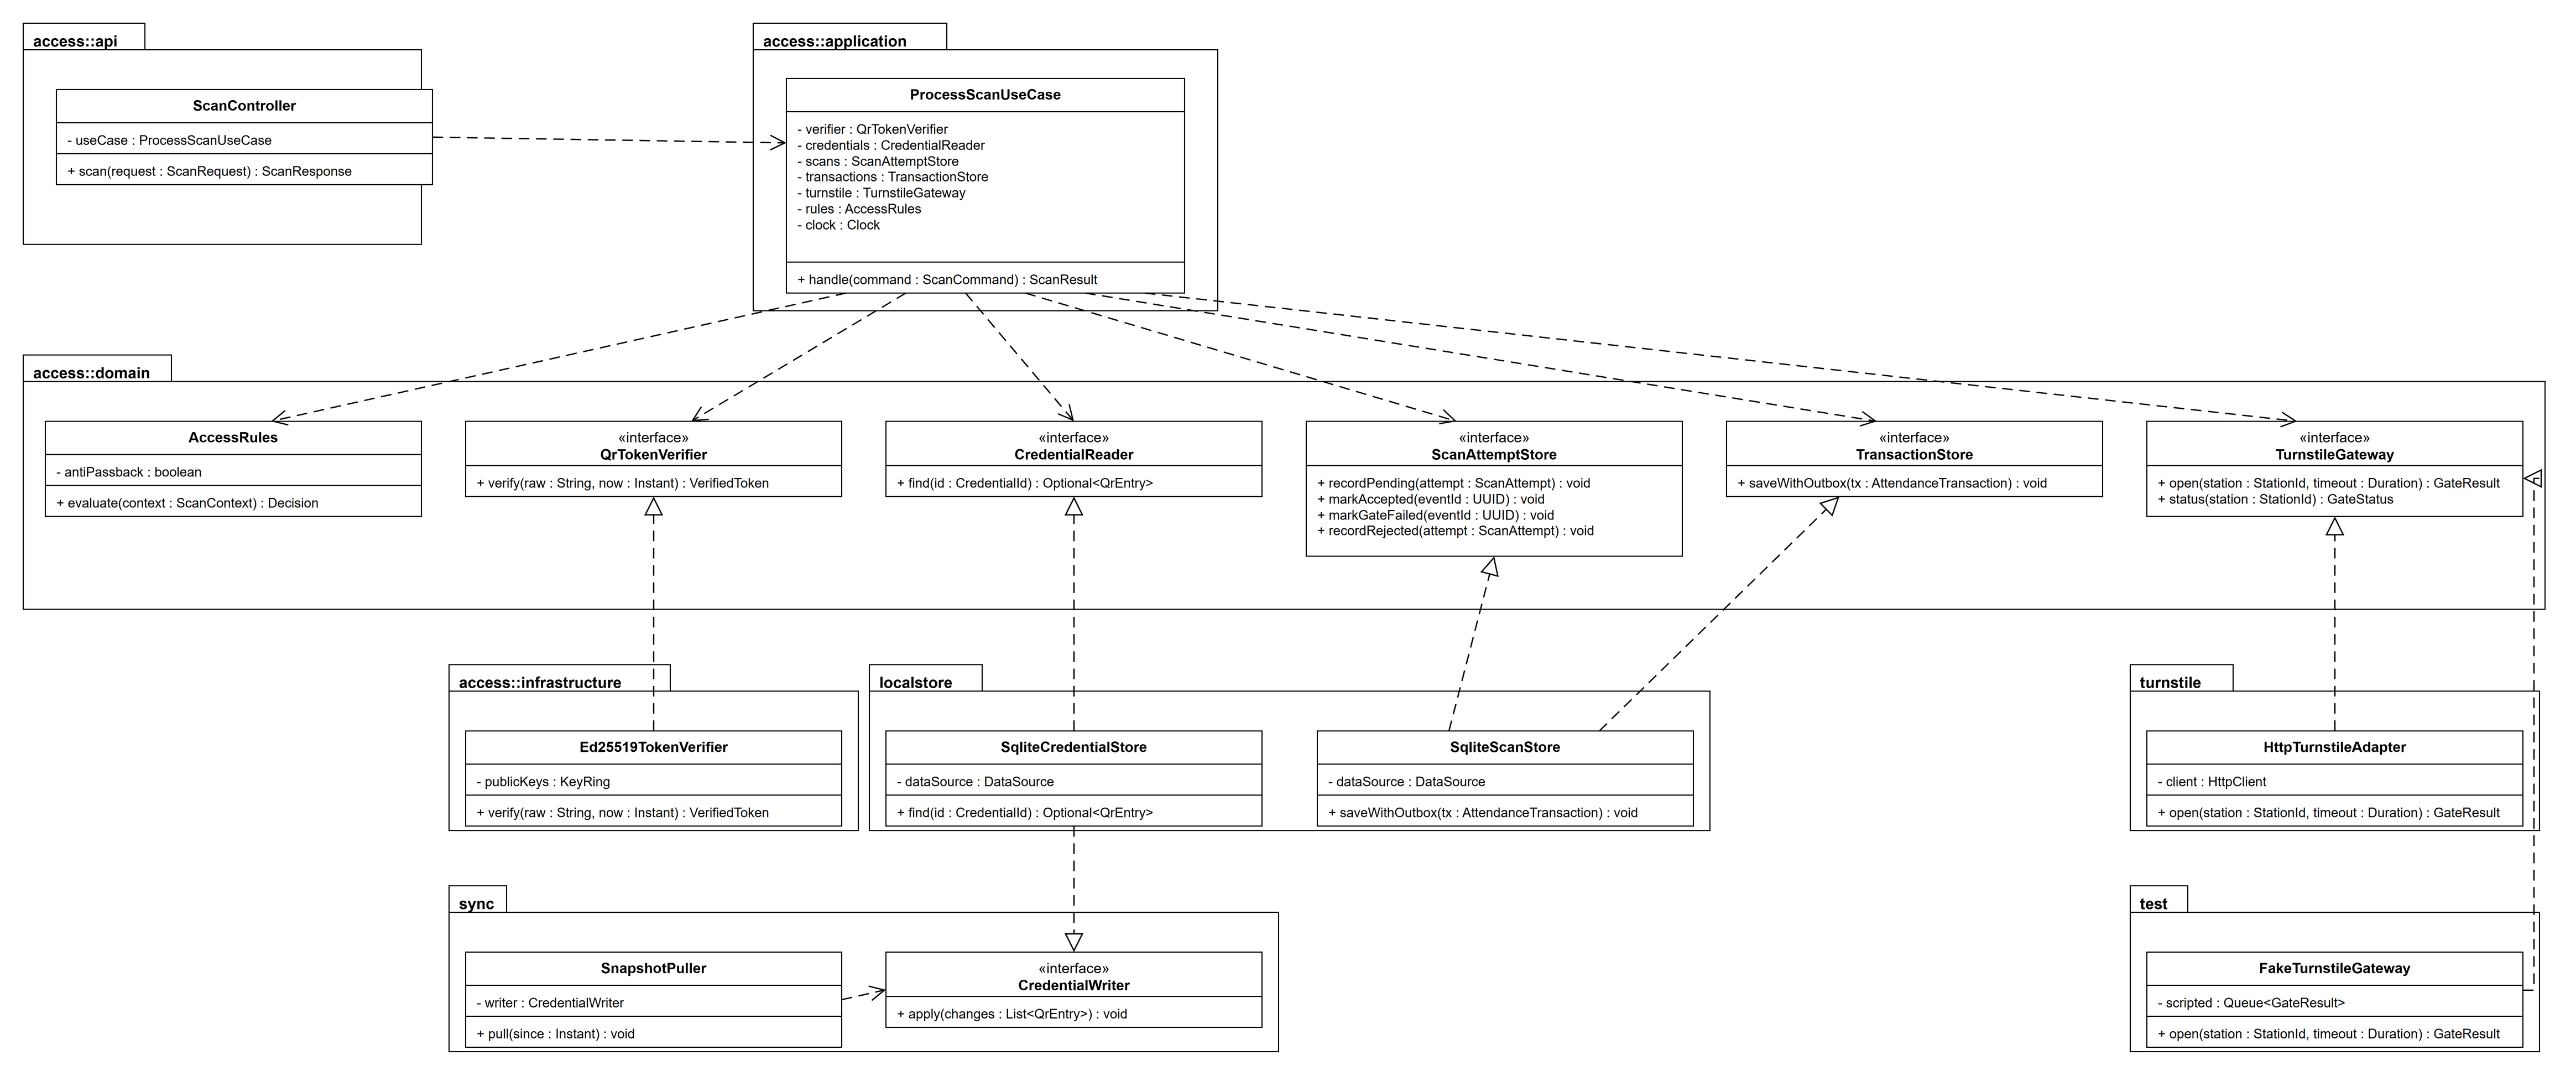
\includegraphics[width=0.92\textheight,height=0.92\textwidth,keepaspectratio]{figures/08_design_principles/class_access_ports.png}}
\caption{Lược đồ lớp các port và adapter của package \texttt{access}}
\label{fig:class-access}
\end{figure}

\subsubsection{Single Responsibility Principle}\label{sec:solid-srp}
\begin{itemize}
    \item \textit{Phát biểu:} Mỗi module, mỗi lớp chỉ có một lý do để thay đổi.
    \item \textit{Áp dụng:} ở mức component, G1, G2, G3 và G4 được tách riêng vì thay đổi vì những lý do khác nhau: quy tắc xác thực, nhà cung cấp cổng xoay, cách lưu trữ và giao thức đồng bộ. Ở mức lớp, \texttt{ProcessScanUseCase} chỉ điều phối luồng quét; quy tắc cho qua nằm trong \texttt{AccessRules}; việc kiểm tra chữ ký và thời hạn mã QR nằm trong \texttt{QrTokenVerifier}.
    \item \textit{Ví dụ:} khi đổi thuật toán ký mã QR, chỉ \texttt{Ed25519TokenVerifier} và adapter ký của C2 thay đổi; khi thêm quy tắc chống quẹt lặp chiều mới, chỉ \texttt{AccessRules} thay đổi.
    \item \textit{Lợi ích:} mỗi thay đổi chỉ cần kiểm thử lại một phạm vi nhỏ. \textit{Nguyên tắc liên quan:} DP-14.
\end{itemize}

\subsubsection{Open/Closed Principle}\label{sec:solid-ocp}
\begin{itemize}
    \item \textit{Phát biểu:} Phần mềm mở cho việc mở rộng nhưng đóng với việc sửa đổi.
    \item \textit{Áp dụng:} các điểm có khả năng thay đổi được đặt sau interface; hành vi mới được thêm bằng một cài đặt mới thay vì sửa mã đang chạy.
    \item \textit{Ví dụ:} thêm nhà cung cấp cổng xoay mới bằng một lớp mới cài đặt \texttt{TurnstileGateway} theo kiểu plugin của Gate Agent (ADR-04), cấu hình chọn adapter cho từng trạm; thêm định dạng xuất báo cáo bằng một lớp xuất báo cáo mới trong C6.
    \item \textit{Lợi ích:} mở rộng được mà không đụng tới mã nghiệp vụ đang chạy ổn định tại cổng. \textit{Nguyên tắc liên quan:} DP-16.
\end{itemize}

\subsubsection{Liskov Substitution Principle}\label{sec:solid-lsp}
\begin{itemize}
    \item \textit{Phát biểu:} Mọi cài đặt của một interface phải thay thế được cho nhau mà không làm sai hành vi của bên sử dụng.
    \item \textit{Áp dụng:} mỗi port có hợp đồng rõ ràng mà mọi cài đặt phải tuân theo. Ví dụ, mọi cài đặt \texttt{TurnstileGateway} phải trả về kết quả hoặc báo lỗi trong giới hạn thời gian chờ được truyền vào, không chặn luồng quét và không ném ngoại lệ ngoài hợp đồng.
    \item \textit{Ví dụ:} \texttt{FakeTurnstileGateway} được dùng thay cho \texttt{HttpTurnstileAdapter} khi kiểm thử các kịch bản cổng không phản hồi hoặc tải giờ giao ca mà không cần phần cứng; đồng hồ cố định (\texttt{java.time.Clock}) được dùng thay đồng hồ hệ thống để kiểm thử việc hết hạn của mã QR.
    \item \textit{Lợi ích:} \texttt{ProcessScanUseCase} được kiểm thử đầy đủ mà không cần thiết bị thật. \textit{Nguyên tắc liên quan:} DP-07, DP-16.
\end{itemize}

\subsubsection{Interface Segregation Principle}\label{sec:solid-isp}
\begin{itemize}
    \item \textit{Phát biểu:} Bên sử dụng không bị buộc phụ thuộc vào những thao tác mà nó không dùng.
    \item \textit{Áp dụng:} các port được thiết kế hẹp theo nhu cầu của từng bên sử dụng, kể cả khi cùng một lớp cài đặt nhiều port.
    \item \textit{Ví dụ:} \texttt{SqliteCredentialStore} cài đặt hai interface: \texttt{CredentialReader} chỉ có thao tác đọc, dành cho G1, và \texttt{CredentialWriter} chỉ có thao tác ghi, dành cho G4. Nhờ đó G1 không thể sửa bản sao credential (DP-04). Tương tự, \texttt{ScanAttemptStore} được tách khỏi \texttt{TransactionStore}; ở Central, interface tra cứu chấm công cho C6 được tách khỏi interface điều chỉnh chấm công của C4.
    \item \textit{Lợi ích:} mỗi bên chỉ thấy những thao tác được phép, phù hợp với nguyên tắc đặc quyền tối thiểu. \textit{Nguyên tắc liên quan:} DP-04, DP-10.
\end{itemize}

\subsubsection{Dependency Inversion Principle}\label{sec:solid-dip}
\begin{itemize}
    \item \textit{Phát biểu:} Module cấp cao không phụ thuộc module cấp thấp; cả hai phụ thuộc vào trừu tượng.
    \item \textit{Áp dụng:} các port được định nghĩa trong tầng \texttt{domain}; các adapter trong \texttt{infrastructure}, \texttt{localstore} và \texttt{turnstile} cài đặt chúng. \texttt{ProcessScanUseCase} chỉ phụ thuộc vào các interface; việc gắn cài đặt cụ thể được thực hiện bằng cơ chế tiêm phụ thuộc của Spring (ADR-10).
    \item \textit{Ví dụ:} trong Hình~\ref{fig:class-access}, mọi quan hệ realization đều hướng từ các package hạ tầng vào \texttt{access::domain}, không có quan hệ nào theo chiều ngược lại.
    \item \textit{Lợi ích:} thay đổi CSDL cục bộ, nhà cung cấp cổng xoay hay API của HR/Payroll không ảnh hưởng tới nghiệp vụ lõi (NFR-MOD-01). \textit{Nguyên tắc liên quan:} DP-16.
\end{itemize}

%==============================================================================
\subsection{Kiểm tra việc tuân thủ nguyên tắc}\label{sec:dp-compliance}
Các nguyên tắc chỉ có giá trị khi được kiểm tra trong quá trình phát triển. Bảng~\ref{tab:dp-compliance} nêu cách kiểm tra từng nguyên tắc.

\begingroup
\small
\renewcommand{\arraystretch}{1.3}
\begin{longtable}{|>{\centering\arraybackslash}p{1.4cm}|>{\raggedright\arraybackslash}p{11.0cm}|>{\raggedright\arraybackslash}p{2.6cm}|}
\caption{Cách kiểm tra việc tuân thủ các nguyên tắc thiết kế}\label{tab:dp-compliance}\\
\hline
\textbf{Nguyên tắc} & \textbf{Cách kiểm tra} & \textbf{ADR liên quan} \\
\hline
\endfirsthead
\hline
\textbf{Nguyên tắc} & \textbf{Cách kiểm tra} & \textbf{ADR liên quan} \\
\hline
\endhead
\hline
\endfoot
\endlastfoot
DP-01 & Kiểm thử dừng Gate Agent ngay sau khi ghi lượt quét rồi khởi động lại; kiểm thử cổng xoay không phản hồi & ADR-03 \\
\hline
DP-02 & Tài khoản CSDL của ứng dụng chỉ có quyền thêm bản ghi trên bảng giao dịch và nhật ký kiểm toán; kiểm thử điều chỉnh chấm công giữ nguyên bản gốc & ADR-03, ADR-08 \\
\hline
DP-03 & Kiểm thử gửi cùng một lô sự kiện hai lần và gửi lại cùng một đợt truyền & ADR-05, ADR-06 \\
\hline
DP-04 & Kiểm thử kiến trúc: chỉ module sở hữu được truy cập lớp lưu trữ của dữ liệu tương ứng & ADR-04, ADR-07 \\
\hline
DP-05 & Kiểm thử kiến trúc: \texttt{gate-agent} không phụ thuộc \texttt{central}; kiểm thử ngắt kết nối WAN trong khi quét & ADR-01 \\
\hline
DP-06 & Review thiết kế: không có lời gọi đồng bộ qua mạng trong luồng quét; theo dõi số bản ghi chờ trong outbox & ADR-05 \\
\hline
DP-07 & Review mã: mọi client gọi ra ngoài phải đặt giới hạn thời gian chờ; kiểm thử với \texttt{FakeTurnstileGateway} trả về hết thời gian chờ & ADR-06 \\
\hline
DP-08 & Kiểm thử vượt ngưỡng mất kết nối ở cả chiều vào và chiều ra & ADR-01 \\
\hline
DP-09 & Kiểm tra endpoint health check và chỉ số vận hành trong kiểm thử triển khai & ADR-07 \\
\hline
DP-10 & Kiểm thử phân quyền theo vai trò và theo phạm vi dữ liệu & ADR-08 \\
\hline
DP-11 & Kiểm thử với mã QR sai chữ ký, hết hạn và đã sử dụng; kiểm thử Gate Agent không có chứng chỉ hợp lệ & ADR-02, ADR-08 \\
\hline
DP-12 & Review hợp đồng dữ liệu gửi sang HR/Payroll; kiểm tra log không chứa mật khẩu, token (NFR-PRI-03) & ADR-08 \\
\hline
DP-13 & Kiểm thử mỗi thao tác nhạy cảm tạo đúng một bản ghi nhật ký kiểm toán & ADR-08 \\
\hline
DP-14 -- DP-16 & Kiểm thử kiến trúc tự động bằng ArchUnit và cơ chế kiểm tra module của Spring Modulith trong CI & ADR-07, ADR-10 \\
\hline
DP-17 & Review mã: không có giá trị ngưỡng, giới hạn thời gian chờ hay lịch viết cứng trong mã & ADR-07 \\
\hline
\end{longtable}
\endgroup
